\PassOptionsToPackage{svgnames}{xcolor}
\documentclass[11pt]{beamer}
%\usetheme{Singapore}
\usepackage[utf8]{inputenc}
\usepackage[english]{babel}
\usepackage{amsmath}
\usepackage{amsfonts}
\usepackage{amssymb}
\usepackage{graphicx}
\usepackage{minted}
\usepackage{pifont}% http://ctan.org/pkg/pifont
\usepackage[skins]{tcolorbox}
\newcommand{\cmark}{\textcolor{green}{\ding{51}}}%
\newcommand{\xmark}{\textcolor{red}{\ding{55}}}%

\newtcbox{\instbox}{enhanced,nobeforeafter,tcbox raise base,boxrule=0.2pt,top=0mm,bottom=0mm,
  right=0mm,left=0mm,arc=1pt,boxsep=1pt,before upper={\vphantom{dlg}}, frame hidden,
  colback=gray!25!white}

\MakeRobust\instbox 

\newtcbox{\regbox}{enhanced,nobeforeafter,tcbox raise base,boxrule=0.2pt,top=0mm,bottom=0mm,
  right=0mm,left=0mm,arc=1pt,boxsep=1pt,before upper={\vphantom{dlg}}, frame hidden,
  colback=Moccasin!75!white}

\MakeRobust\regbox
 
\newcommand{\acr}{reg.ac}
\newcommand{\inst}[1]{\instbox{\texttt{#1}}} % to display instructions
\newcommand{\reg}[1]{\regbox{\texttt{#1}}} % to register names or related 
%\author{}
\title{Discussing speculation attacks}
%\setbeamercovered{transparent} 
\setbeamertemplate{navigation symbols}{} 
%\logo{} 
\institute{uSC SIG / RISCV} 
%\date{} 
%\subject{} 
\begin{document}

\maketitle

\section{Introduction}


\begin{frame}[fragile]
    \frametitle{Introduction to Spectre-PHT in $1$ slide}

    \begin{minted}[escapeinside=||]{c}
if (|\textcolor{ForestGreen}{x < array1\_size}|) {
    y = |\textcolor{blue}{array2[}||\textcolor{red}{array1[x]}||\textcolor{blue}{ * 4096]}|;
}
    \end{minted}

    \begin{block}{Steps}
        \begin{enumerate}
            \item Mistrain the \textcolor{ForestGreen}{branch prediction} mechanism to trigger speculative execution on an incorrect condition.
            \item Read the \textcolor{red}{secret} at address \textcolor{red}{\texttt{array1} + x}, for an arbitrary \textcolor{red}{x}.
            \item \textbf{Write} (part of) the \textcolor{red}{secret} in the tag field of the cache memory with a \textcolor{blue}{\textbf{read} memory access}.
            \item Read the \textcolor{red}{secret} with a cache timing analysis.
        \end{enumerate}
        
    \end{block}

    \begin{center}
        \textbf{Step $3$ and $4$ can be replaced with any covert channel !}
    \end{center}

\end{frame}

\section{Countermeasures}
\frame{\sectionpage}

\begin{frame}
    \frametitle{Disclaimers}

    \begin{itemize}
        \item No speculative attack has been reported in the wild.
        \item Some papers only consider cache based covert channels, this is not enough for an actual solution.
        \item Speculative attacks can be solved with hardware modifications only. $\rightarrow$ no RISCV ISA extension \textit{required}, but may help performances.
    \end{itemize}
        

\end{frame}

\begin{frame}
    \frametitle{Strategies from a bird's view}

    \begin{enumerate}
        \item Add dedicated microstructures to deal with speculation. Ex: Invispec speculatively load data in a \textit{speculation buffer} instead of the cache.
        \item Defer sensitive operations to prevent speculatively executing them.
    \end{enumerate}

    In the \textit{defer} strategy, countermeasures often implement hardware taint tracking to choose what instructions to delay.
    
    \begin{block}{A lot of questions}
        What are the costs (area, time, power) of these strategies ?
        Are these costs definitive or implementation dependent ?
    \end{block}

\end{frame}


% reported costs

\begin{frame}
    \frametitle{Self-reported slowdown\footnote{After a quick read, without judging the security merits nor the veracity of reported slowdowns.}}

    

    \begin{center}
        \begin{tabular}{|c | c  | c |}
        \hline Countermeasure & Slowdown & Main strategy\\
        \hline InvisiSpec & $21\%-72\%$  & Structures \\
        STT & $8\%-15\%$ & Defer \& tainting \\
        SafeSpec & $-3\%$ &  Structures \\
        NDA &  $10\%-125\%$ & Defer \& tainting\\
        Dolma &  $9\%-63\%$ & Defer \& tainting\\
        SpecShield & $10\%-73\%$ & Defer \& tainting \\
        SpecTerminator & $2.6\%-6\%$ & Defer \& tainting \\ 
        \hline
        \end{tabular}
    \end{center}

\end{frame}

\begin{frame}
    \frametitle{NDA self-evaluation}

    \begin{figure}
        \centering
        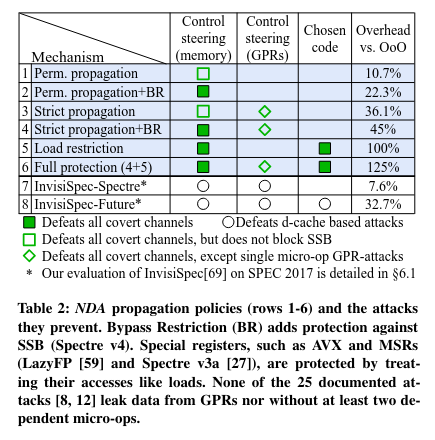
\includegraphics[width=.6\textwidth]{NDA_eval.png}
    \end{figure}
    

\end{frame}


\end{document}